% !TeX encoding = UTF-8
% !TeX spellcheck = en_GB
\section{Logging}
\subsection{Fluentd}
\subsubsection{Decision Log}

%In order to manage difficulties like logs scattered across multiple sources or disparate log formats we decided to use Fluentd.
Fluentd is an open source data collector which processes the data from various sources, making it easier to manage and analyze.
The following aspects show why we used Fluentd:
\begin{itemize}
	\item \textbf{Unified Logging Layer:} Provides a unified platform for collecting, transforming, and routing logs from diverse sources.
	\item \textbf{Data Agnosticism:} Seamlessly collects and processes data in a unified format regardless of the data source.
	\item \textbf{Configurable Routing:} Effortlessly configure log routing based on application or service, directing logs to specific destinations for centralized storage and analysis.
	\item \textbf{Flexibility:} Enables us to send data from any source to any destination.
\end{itemize}

\subsubsection{Implementation of Fluentd}

A diagram describing our use and implementation of Fluentd can be seen in figure \ref{fig:logging2}.
\begin{figure}[H]
	\centering
	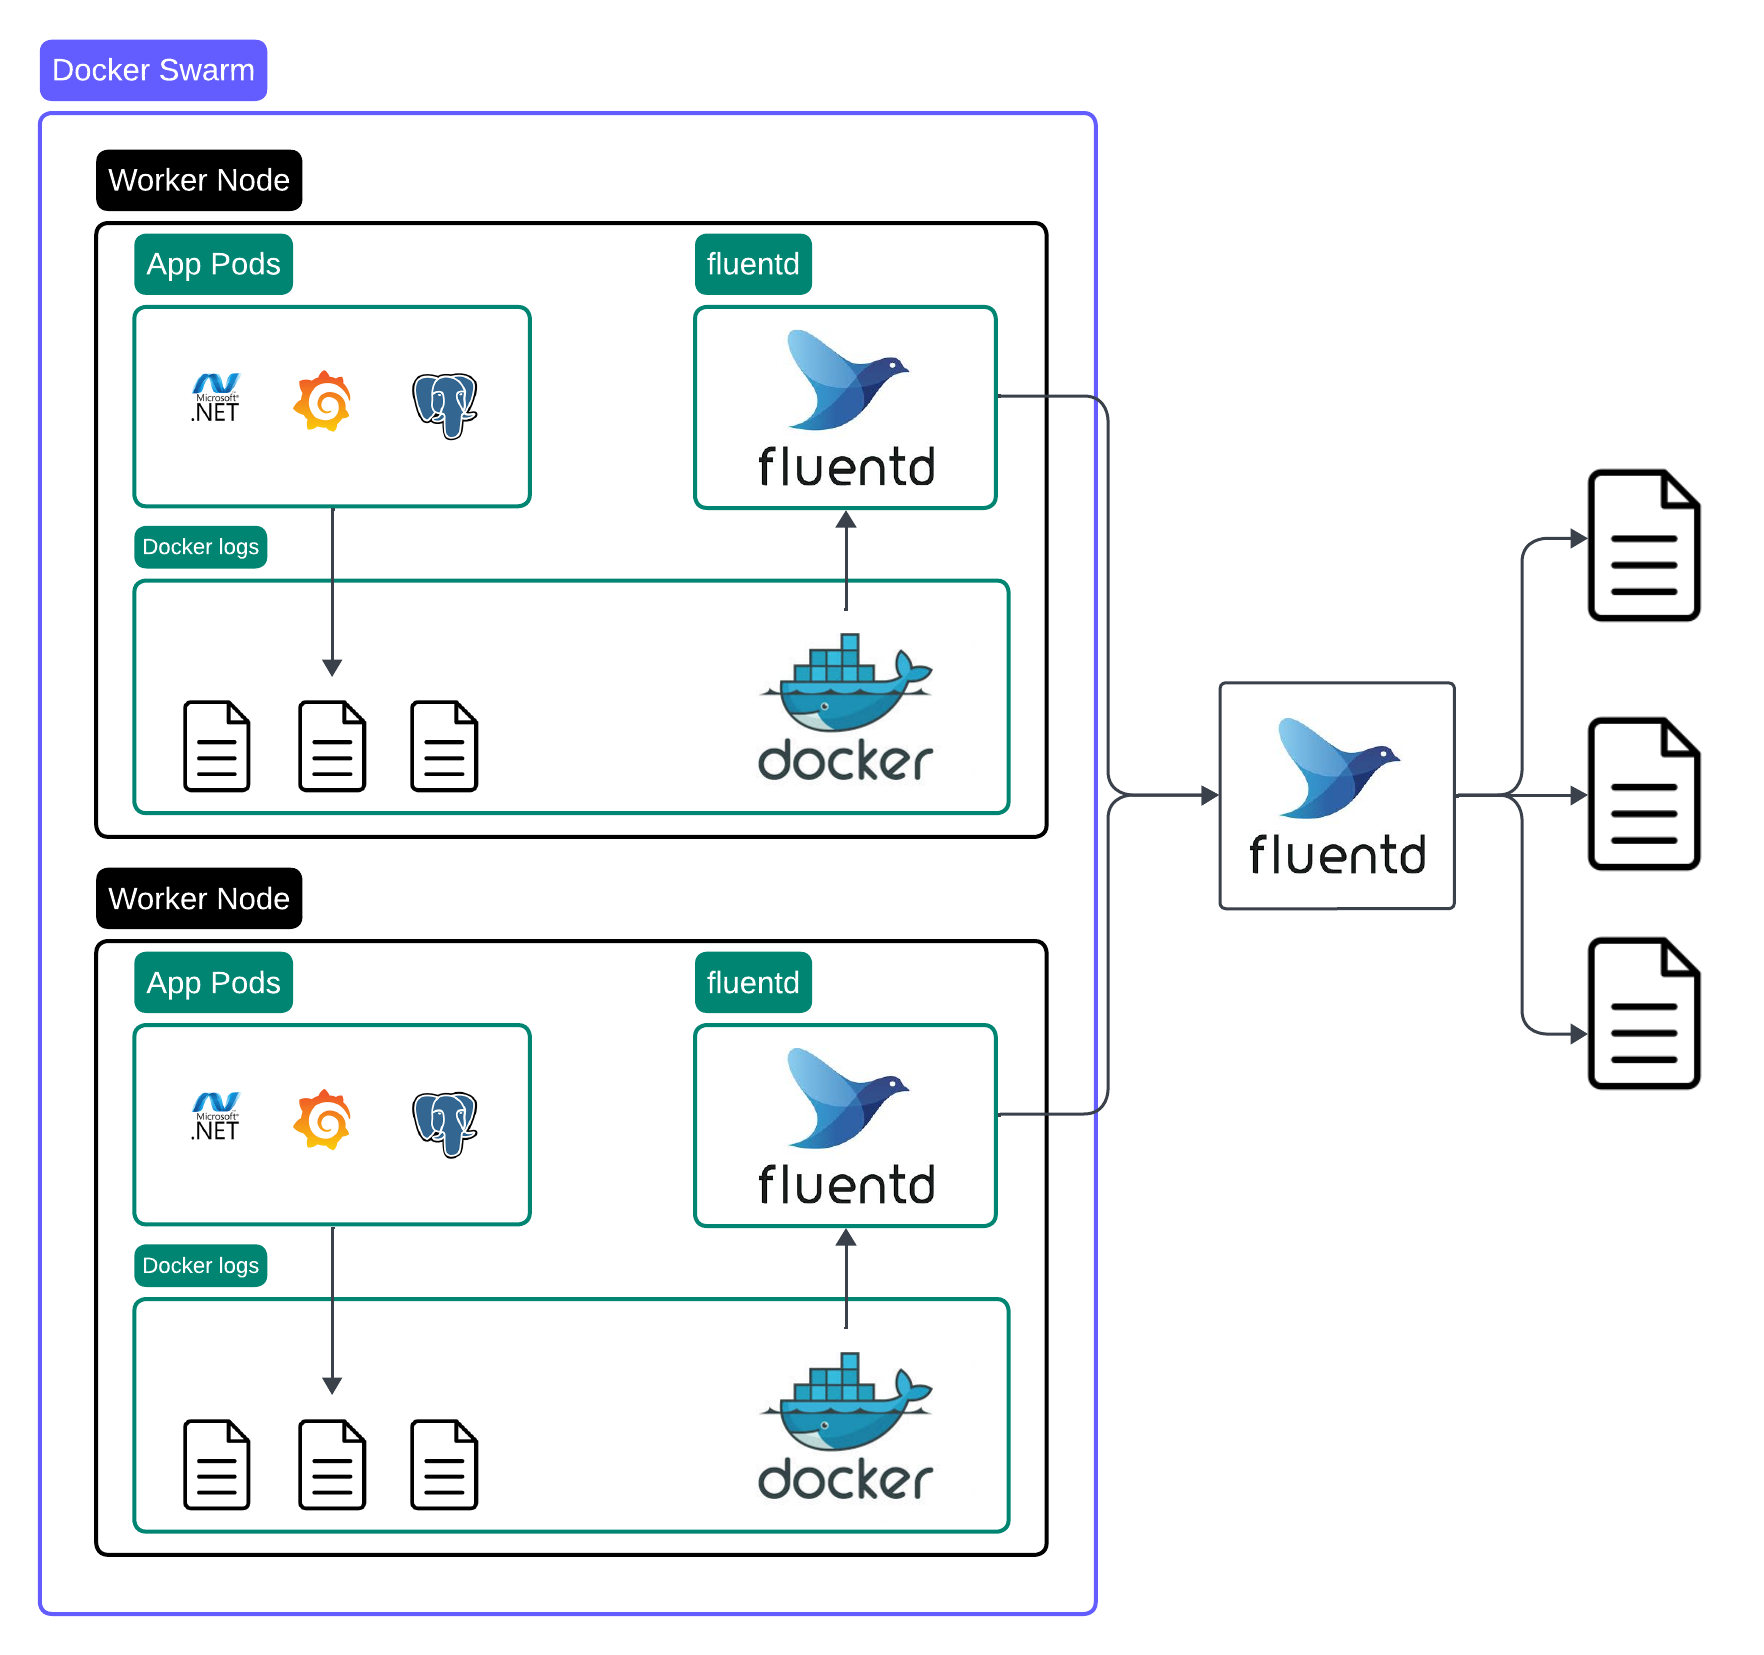
\includegraphics[width=1\textwidth]{Logging2.png}
	\caption{Diagram describing our implementation of Fluentd}
	\label{fig:logging2}
\end{figure}

\subsubsection*{Fluentd Configuration}

Fluentd is configured to listen for incoming log data.%via the forward input plugin on port 24224.
Log data from different sources is matched using the match directive.%which specifies the destination path and format for the corresponding log data.
Log data is buffered using the buffer directive to handle data spikes or network outages.%, ensuring reliable log collection.

\subsubsection*{Docker Compose Configuration}

A Fluentd container is defined %using the fluent/fluentd:v1.12-debian image.
and each service in the Docker Compose file depends on the Fluentd service for logging.
%Logging is configured to use Fluentd as the logging driver, with specific options (fluentd-async-connect, fluentd-retry-wait, fluentd-max-retries) to ensure reliable log transmission.
%Each service specifies a unique tag to route log data to the appropriate destination, which in our case are simple log files.

